% answers.tex —— 2009 年·普通高等学校招生考试·辽宁卷·理科 · 参考答案与详细解析片段
% 由 tools/generate_projects.py 依来源总账自 2009/2009_数学真题_辽宁理_试题.md + 2009/2009_数学真题_辽宁理_解析正文.md + 2009/2009_数学真题_辽宁理_答案要点.md 生成，勿手改（改源 MD 后重跑）


\begin{gktip}
固定候选 PDF 仅含题面，无答案、解析和评分标准，原卷亦未标分值；以下为非官方编者独立推导，官方答案字段为空。题面文字层只作定位，分数、根号、上下标与六幅图均以 600 dpi 原页复核。第 19 题原页「向一目射击」按「向一目标射击」理解。
\end{gktip}

\begin{answer}
\gksolhead{1}{}

\textbf{题目}：

已知集合 $M=\{x\mid -3<x\leqslant5\}$，$N=\{x\mid -5<x<5\}$，则 $M\cap N=$（　）

（A）$\{x\mid -5<x<5\}$

（B）$\{x\mid -3<x<5\}$

（C）$\{x\mid -5<x\leqslant5\}$

（D）$\{x\mid -3<x\leqslant5\}$

\Needspace{4\baselineskip}
\textbf{解析}

\Needspace{5\baselineskip}
$M$ 是左开右闭区间 $(-3,5]$，$N$ 是开区间 $(-5,5)$。交集要求同时满足两个不等式，即

\nopagebreak[4]
\[-3<x\leqslant5\quad\text{\text{且}}\quad-5<x<5 .\]

\Needspace{5\baselineskip}
后一条件比前一条件在右端更严（$x<5$ 强于 $x\leqslant5$），左端则以 $-3<x$ 为准，故

\nopagebreak[4]
\[M\cap N=\{x\mid -3<x<5\},\]

选 B。注意 $x=5$ 属于 $M$ 但不属于 $N$，故不能取到 $5$。

\gkanswer{答案：B。}

\end{answer}
\begin{answer}
\gksolhead{2}{}

\textbf{题目}：

已知复数 $z=1-2\mathrm i$，那么 $\frac1z=$（　）

（A）$\frac{\sqrt5}{5}+\frac{2\sqrt5}{5}\mathrm i$

（B）$\frac{\sqrt5}{5}-\frac{2\sqrt5}{5}\mathrm i$

（C）$\frac15+\frac25\mathrm i$

（D）$\frac15-\frac25\mathrm i$

\Needspace{4\baselineskip}
\textbf{解析}

\Needspace{5\baselineskip}
分子分母同乘 $1+2\mathrm i$：

\nopagebreak[4]
\[\frac1{1-2\mathrm i}
=\frac{1+2\mathrm i}{(1-2\mathrm i)(1+2\mathrm i)}
=\frac{1+2\mathrm i}{1+4}
=\frac{1+2\mathrm i}{5}
=\frac15+\frac25\mathrm i,\]

选 C。

\gkanswer{答案：C。}

\end{answer}
\begin{answer}
\gksolhead{3}{}

\textbf{题目}：

平面向量 $\boldsymbol a$ 与 $\boldsymbol b$ 的夹角为 $60^\circ$，$\boldsymbol a=(2,0)$，$|\boldsymbol b|=1$，则 $|\boldsymbol a+2\boldsymbol b|=$（　）

（A）$\sqrt3$

（B）$2\sqrt3$

（C）$4$

（D）$12$

\Needspace{4\baselineskip}
\textbf{解析}

\Needspace{5\baselineskip}
由 $|\boldsymbol a|=2$、$|\boldsymbol b|=1$ 及夹角 $60^\circ$，

\nopagebreak[4]
\[\boldsymbol a\cdot\boldsymbol b
=|\boldsymbol a||\boldsymbol b|\cos60^\circ
=2\times1\times\frac12=1 .\]

\Needspace{5\baselineskip}
于是

\nopagebreak[4]
\[|\boldsymbol a+2\boldsymbol b|^2
=\boldsymbol a\cdot\boldsymbol a+4\boldsymbol a\cdot\boldsymbol b
+4\boldsymbol b\cdot\boldsymbol b
=4+4+4=12,\]

故 $|\boldsymbol a+2\boldsymbol b|=2\sqrt3$，选 B。这里 $4\boldsymbol b\cdot\boldsymbol b=4|\boldsymbol b|^2=4$。

\gkanswer{答案：B。}

\end{answer}
\begin{answer}
\gksolhead{4}{}

\textbf{题目}：

已知圆 $C$ 与直线 $x-y=0$ 及 $x-y-4=0$ 都相切，圆心在直线 $x+y=0$ 上，则圆 $C$ 的方程为（　）

（A）$(x+1)^2+(y-1)^2=2$

（B）$(x-1)^2+(y+1)^2=2$

（C）$(x-1)^2+(y-1)^2=2$

（D）$(x+1)^2+(y+1)^2=2$

\Needspace{4\baselineskip}
\textbf{解析}

\Needspace{5\baselineskip}
两条平行线 $x-y=0$ 与 $x-y-4=0$ 的距离为

\nopagebreak[4]
\[d=\frac{|0-(-4)|}{\sqrt{1^2+(-1)^2}}
=\frac4{\sqrt2}=2\sqrt2 .\]

圆与两线都相切，直径等于两线间距，故半径 $r=\sqrt2$。

\Needspace{5\baselineskip}
圆心到两线距离相等，必在两条平行线的中位线 $x-y-2=0$ 上；又圆心在 $x+y=0$ 上。联立

\nopagebreak[4]
\[\begin{cases}x-y-2=0,\\ x+y=0,\end{cases}\]

\Needspace{5\baselineskip}
解得 $x=1$、$y=-1$，圆心为 $(1,-1)$。所求圆方程为

\nopagebreak[4]
\[(x-1)^2+(y+1)^2=2,\]

选 B。

\gkanswer{答案：B。}

\end{answer}
\begin{answer}
\gksolhead{5}{}

\textbf{题目}：

从 $5$ 名男医生、$4$ 名女医生中选 $3$ 名医生组成一个医疗小分队，要求其中男、女医生都有，则不同的组队方案共有（　）

（A）$70$ 种

（B）$80$ 种

（C）$100$ 种

（D）$140$ 种

\Needspace{4\baselineskip}
\textbf{解析}

\Needspace{5\baselineskip}
共有 $5+4=9$ 名医生，任选 $3$ 名的选法为 $\mathrm C_9^3=84$。不满足“男、女都有”的情形只有两种：全为男医生或全为女医生，分别为

\nopagebreak[4]
\[\mathrm C_5^3=10,\qquad \mathrm C_4^3=4 .\]

\Needspace{5\baselineskip}
故所求方案数为

\nopagebreak[4]
\[84-10-4=70,\]

选 A。

\gkanswer{答案：A。}

\end{answer}
\begin{answer}
\gksolhead{6}{}

\textbf{题目}：

设等比数列 $\{a_n\}$ 的前 $n$ 项和为 $S_n$，若 $\frac{S_6}{S_3}=3$，则 $\frac{S_9}{S_6}=$（　）

（A）$2$

（B）$\frac73$

（C）$\frac83$

（D）$3$

\Needspace{4\baselineskip}
\textbf{解析}

\Needspace{5\baselineskip}
等比数列中

\nopagebreak[4]
\[S_6=S_3+q^3S_3=S_3(1+q^3).\]

\Needspace{5\baselineskip}
由 $\frac{S_6}{S_3}=3$ 得 $1+q^3=3$，即 $q^3=2$。于是 $q^6=4$、$q^9=8$，且

\nopagebreak[4]
\[\frac{S_9}{S_6}
=\frac{1-q^9}{1-q^6}
=\frac{1-8}{1-4}
=\frac73,\]

选 B。也可写成 $S_9=S_3(1+q^3+q^6)=S_3(1+2+4)=7S_3$，而 $S_6=3S_3$，比值同为 $\frac73$。

\gkanswer{答案：B。}

\end{answer}
\begin{answer}
\gksolhead{7}{}

\textbf{题目}：

曲线 $y=\frac{x}{x-2}$ 在点 $(1,-1)$ 处的切线方程为（　）

（A）$y=x-2$

（B）$y=-3x+2$

（C）$y=2x-3$

（D）$y=-2x+1$

\Needspace{4\baselineskip}
\textbf{解析}

\Needspace{5\baselineskip}
由商的求导法则，

\nopagebreak[4]
\[y'=\frac{1\cdot(x-2)-x\cdot1}{(x-2)^2}
=-\frac{2}{(x-2)^2}.\]

\Needspace{5\baselineskip}
在 $x=1$ 处，$y'=-2$，故切线斜率为 $-2$。切点为 $(1,-1)$，切线方程为

\nopagebreak[4]
\[y+1=-2(x-1),\]

即 $y=-2x+1$，选 D。

\gkanswer{答案：D。}

\end{answer}
\begin{answer}
\gksolhead{8}{}

\textbf{题目}：

已知函数 $f(x)=A\cos(\omega x+\varphi)$ 的图象如图所示，$f\left(\frac{\pi}{2}\right)=-\frac23$，则 $f(0)=$（　）

（A）$-\frac23$

（B）$\frac23$

（C）$-\frac12$

（D）$\frac12$
\nopagebreak[4]
\begin{center}% 2009 年辽宁卷理科第 8 题：f(x)=Acos(ωx+φ) 的图象。
% 来源 PDF：普通高考/2009/2009辽宁理.pdf，SHA256 5ae9708acfe7def5bddd60a34d1474cfa2e2c20a39d130255e0e4393093accad
% 原页：第 1 页（A3 三栏）第 1 栏下部，印刷页 537。
% 重绘依据：曲线在 x=7π/12 与 x=11π/12 处与 x 轴相交，两零点之间为正值峰；
%   故半周期为 π/3、ω=3。又 x=π/2 处函数值为 −2/3（虚线标出），由此定出振幅，
%   进而 f(0)=2/3。原图只画峰附近一段，y 轴在左侧。
\begin{tikzpicture}[scale=1.15, semithick, >=Stealth,
  every node/.style={inner sep=1.5pt, font=\small}]
  \draw[->] (-0.55,0) -- (3.35,0) node[right] {$x$};
  \draw[->] (0,-1.35) -- (0,1.32) node[above] {$y$};
  \node[below left] at (0,0) {$O$};
  \draw[domain=1.22:3.12, samples=240, smooth, thick]
    plot (\x,{0.9428*sin(deg(3*(\x-1.8326)))});
  \draw[densely dashed] (0,-0.6667) -- (1.5708,-0.6667);
  \draw[densely dashed] (1.5708,-0.6667) -- (1.5708,0);
  \draw (1.8326,0.09) -- (1.8326,-0.09);
  \draw (2.8798,0.09) -- (2.8798,-0.09);
  \node[left] at (-0.06,-0.6667) {$-\frac23$};
  \node[above] at (1.5708,0.04) {$\frac{\pi}{2}$};
  \node[below] at (1.8326,-0.72) {$\frac{7\pi}{12}$};
  \node[below] at (2.8798,-0.72) {$\frac{11\pi}{12}$};
\end{tikzpicture}
\end{center}
\nopagebreak[4]
\Needspace{4\baselineskip}
\textbf{解析}

\Needspace{5\baselineskip}
图中曲线在 $x=\frac{7\pi}{12}$ 与 $x=\frac{11\pi}{12}$ 处与 $x$ 轴相交，且两零点之间为正峰，因此这两点是相邻零点，半周期为

\nopagebreak[4]
\[\frac{T}{2}=\frac{11\pi}{12}-\frac{7\pi}{12}=\frac{\pi}{3},\]

故 $T=\frac{2\pi}{3}$，$\omega=\frac{2\pi}{T}=3$。

\Needspace{5\baselineskip}
设 $f(x)=A\cos(3x+\varphi)$。由 $f\left(\frac{7\pi}{12}\right)=0$ 得

\nopagebreak[4]
\[\cos\left(\frac{7\pi}{4}+\varphi\right)=0
\ \Longrightarrow\ \frac{7\pi}{4}+\varphi=\frac{\pi}{2}+k\pi .\]

\Needspace{5\baselineskip}
取 $k=1$ 得 $\varphi=-\frac{\pi}{4}$。再由

\nopagebreak[4]
\[f\left(\frac{\pi}{2}\right)
=A\cos\left(\frac{3\pi}{2}-\frac{\pi}{4}\right)
=A\cos\frac{5\pi}{4}
=-\frac{\sqrt2}{2}A
=-\frac23,\]

\Needspace{5\baselineskip}
得 $A=\frac{2\sqrt2}{3}$。于是

\nopagebreak[4]
\[f(0)=A\cos\left(-\frac{\pi}{4}\right)
=\frac{2\sqrt2}{3}\cdot\frac{\sqrt2}{2}
=\frac23,\]

选 B。数值上 $A\approx0.943$，与图中峰高约为 $1$ 相符。

\gkanswer{答案：B。}

\end{answer}
\begin{answer}
\gksolhead{9}{}

\textbf{题目}：

已知偶函数 $f(x)$ 在区间 $[0,+\infty)$ 单调增加，则满足 $f(2x-1)<f\left(\frac13\right)$ 的 $x$ 取值范围是（　）

（A）$\left(\frac13,\frac23\right)$

（B）$\left[\frac13,\frac23\right)$

（C）$\left(\frac12,\frac23\right)$

（D）$\left[\frac12,\frac23\right)$

\Needspace{4\baselineskip}
\textbf{解析}

\Needspace{5\baselineskip}
$f$ 为偶函数，故 $f\left(\frac13\right)=f\left(-\frac13\right)$，且 $f$ 在 $[0,+\infty)$ 上单调增加。于是

\nopagebreak[4]
\[f(2x-1)<f\left(\frac13\right)
\iff |2x-1|<\frac13 .\]

\Needspace{5\baselineskip}
解绝对值不等式：

\nopagebreak[4]
\[-\frac13<2x-1<\frac13
\iff \frac23<2x<\frac43
\iff \frac13<x<\frac23,\]

选 A。区间两端均取不到，因为题中为严格不等式。

\gkanswer{答案：A。}

\end{answer}
\begin{answer}
\gksolhead{10}{}

\textbf{题目}：

某店一个月的收入和支出总共记录了 $N$ 个数据 $a_1,a_2,\cdots,a_N$，其中收入记为正数，支出记为负数．该店用下边的程序框图计算月总收入 $S$ 和月净盈利 $V$，那么在图中空白的判断框和处理框中，应分别填入下列四个选项中的（　）

（A）$A>0$，$V=S-T$

（B）$A<0$，$V=S-T$

（C）$A>0$，$V=S+T$

（D）$A<0$，$V=S+T$
\nopagebreak[4]
\begin{center}% 2009 年辽宁卷理科第 10 题：计算月总收入 S 与月净盈利 V 的程序框图。
% 来源 PDF：普通高考/2009/2009辽宁理.pdf，SHA256 5ae9708acfe7def5bddd60a34d1474cfa2e2c20a39d130255e0e4393093accad
% 原页：第 1 页（A3 三栏）第 2 栏上部，印刷页 537。
% 重绘依据：开始 → 输入 N,a1,...,aN → k=1,S=0,T=0 → A=ak → 判断框（原页空白）：
%   否（左）T=T+A，是（右）S=S+A；两路汇合后判断 k<N：是（右）k=k+1 回到 A=ak，
%   否（下）输出 S,V → 结束。判断框内的条件在原页留空，由选项填入。
\begin{tikzpicture}[scale=0.82, semithick, >=Stealth,
  every node/.style={inner sep=3pt, font=\small}]
  \node (start) at (0,0) [draw, rounded corners=4pt, minimum width=2.1cm, minimum height=0.6cm] {开始};
  \node (input) at (0,-1.3) [draw, trapezium, trapezium left angle=75, trapezium right angle=105,
    minimum width=4.9cm, minimum height=0.72cm] {输入 $N,\,a_1,\,a_2,\,\cdots,\,a_N$};
  \node (init) at (0,-2.75) [draw, minimum width=4.0cm, minimum height=0.7cm] {$k=1,\ S=0,\ T=0$};
  \node (ak) at (0,-4.05) [draw, minimum width=1.75cm, minimum height=0.62cm] {$A=a_k$};
  \node (cond) at (0,-5.55) [draw, diamond, aspect=2.4, minimum width=3.3cm, minimum height=1.1cm] {};
  \node (t) at (-2.75,-7.1) [draw, minimum width=2.0cm, minimum height=0.62cm] {$T=T+A$};
  \node (s) at (2.75,-7.1) [draw, minimum width=2.0cm, minimum height=0.62cm] {$S=S+A$};
  \node (kn) at (0,-8.9) [draw, diamond, aspect=2.2, minimum width=2.5cm, minimum height=1.0cm] {$k<N$};
  \node (inc) at (5.0,-8.05) [draw, minimum width=2.0cm, minimum height=0.62cm] {$k=k+1$};
  \node (out) at (0,-10.55) [draw, trapezium, trapezium left angle=75, trapezium right angle=105,
    minimum width=2.7cm, minimum height=0.68cm] {输出 $S,\,V$};
  \node (end) at (0,-11.8) [draw, rounded corners=4pt, minimum width=2.0cm, minimum height=0.6cm] {结束};
  \coordinate (merge) at (0,-8.0);

  \draw[->] (start) -- (input);
  \draw[->] (input) -- (init);
  \draw[->] (init) -- (ak);
  \draw[->] (ak) -- (cond);
  \draw[->] (cond.west) -| node[pos=0.28, above] {否} (t.north);
  \draw[->] (cond.east) -| node[pos=0.28, above] {是} (s.north);
  \draw (t.south) -- (t.south |- merge) -- (merge);
  \draw (s.south) -- (s.south |- merge) -- (merge);
  \draw[->] (merge) -- (kn.north);
  \draw[->] (kn.east) -- node[below=2pt, pos=0.45] {是} (inc.west);
  \draw[->] (inc.north) |- (ak.east);
  \draw[->] (kn.south) -- node[right=2pt, pos=0.45] {否} (out.north);
  \draw[->] (out) -- (end);
\end{tikzpicture}
\end{center}
\nopagebreak[4]
\Needspace{4\baselineskip}
\textbf{解析}

$S$ 只累加正数（收入），$T$ 只累加负数（支出）。因此判断框要区分当前数据 $A=a_k$ 的正负：应填 $A>0$。

\begin{itemize}
\item 判断为“是”时执行 $S=S+A$，把收入累加到 $S$；
\item 判断为“否”时执行 $T=T+A$，把支出（负数）累加到 $T$。
\end{itemize}

\Needspace{5\baselineskip}
循环结束后 $S$ 为月总收入，月净盈利应为收入与支出之和，即处理框填

\nopagebreak[4]
\[V=S+T .\]

故选 C。

\gkanswer{答案：C。}

\end{answer}
\begin{answer}
\gksolhead{11}{}

\textbf{题目}：

正六棱锥 $P-ABCDEF$ 中，$G$ 为 $PB$ 的中点，则三棱锥 $D-GAC$ 与三棱锥 $P-GAC$ 体积之比为（　）

（A）$1:1$

（B）$1:2$

（C）$2:1$

（D）$3:2$

\Needspace{4\baselineskip}
\textbf{解析}

\Needspace{5\baselineskip}
设正六棱锥底面边长为 $2$、高为 $h$。取底面中心为原点，使

\nopagebreak[4]
\[A(2,0,0),\quad B(1,\sqrt3,0),\quad C(-1,\sqrt3,0),\quad D(-2,0,0),\quad P(0,0,h).\]

\Needspace{5\baselineskip}
这是边长为 $2$ 的正六边形的一组标准坐标。$G$ 为 $PB$ 的中点，故

\nopagebreak[4]
\[G\left(\frac12,\frac{\sqrt3}{2},\frac h2\right).\]

\Needspace{5\baselineskip}
三棱锥 $D-GAC$ 的体积为

\nopagebreak[4]
\[V_{D-GAC}
=\frac16\left|\det(\overrightarrow{DA},\overrightarrow{DC},\overrightarrow{DG})\right| .\]

\Needspace{5\baselineskip}
其中

\nopagebreak[4]
\[\overrightarrow{DA}=(4,0,0),\quad
\overrightarrow{DC}=(1,\sqrt3,0),\quad
\overrightarrow{DG}=\left(\frac52,\frac{\sqrt3}{2},\frac h2\right).\]

\Needspace{5\baselineskip}
按第三列展开行列式：

\nopagebreak[4]
\[\det
\begin{pmatrix}
4&0&0\\
1&\sqrt3&0\\
\frac52&\frac{\sqrt3}{2}&\frac h2
\end{pmatrix}
=4\cdot\sqrt3\cdot\frac h2=2\sqrt3 h,\]

故 $V_{D-GAC}=\frac{\sqrt3 h}{3}$。

\Needspace{5\baselineskip}
三棱锥 $P-GAC$ 的体积为

\nopagebreak[4]
\[V_{P-GAC}
=\frac16\left|\det(\overrightarrow{PA},\overrightarrow{PC},\overrightarrow{PG})\right| .\]

\Needspace{5\baselineskip}
其中

\nopagebreak[4]
\[\overrightarrow{PA}=(2,0,-h),\quad
\overrightarrow{PC}=(-1,\sqrt3,-h),\quad
\overrightarrow{PG}=\left(\frac12,\frac{\sqrt3}{2},-\frac h2\right).\]

\Needspace{5\baselineskip}
计算混合积：

\nopagebreak[4]
\[\det
\begin{pmatrix}
2&0&-h\\
-1&\sqrt3&-h\\
\frac12&\frac{\sqrt3}{2}&-\frac h2
\end{pmatrix}
=2\left(-\frac{\sqrt3 h}{2}+\frac{\sqrt3 h}{2}\right)
+(-h)\left(-\frac{\sqrt3}{2}-\frac{\sqrt3}{2}\right)
=\sqrt3 h,\]

\Needspace{5\baselineskip}
故 $V_{P-GAC}=\frac{\sqrt3 h}{6}$。于是

\nopagebreak[4]
\[V_{D-GAC}:V_{P-GAC}=\frac{\sqrt3 h}{3}:\frac{\sqrt3 h}{6}=2:1,\]

选 C。

\gkanswer{答案：C。}

\end{answer}
\begin{answer}
\gksolhead{12}{}

\textbf{题目}：

若 $x_1$ 满足 $2x+2^x=5$，$x_2$ 满足 $2x+2\log_2(x-1)=5$，则 $x_1+x_2=$（　）

（A）$\frac52$

（B）$3$

（C）$\frac72$

（D）$4$

\Needspace{4\baselineskip}
\textbf{解析}

\Needspace{5\baselineskip}
由 $2x_1+2^{x_1}=5$ 得

\nopagebreak[4]
\[2^{x_1}=5-2x_1 .\]

\Needspace{5\baselineskip}
令 $u=\frac72-x_1$，则 $u-1=\frac52-x_1$。由上式得

\nopagebreak[4]
\[2^{x_1-1}=\frac{5-2x_1}{2}=\frac52-x_1=u-1,\]

\Needspace{5\baselineskip}
两边取以 $2$ 为底的对数：

\nopagebreak[4]
\[\log_2(u-1)=x_1-1 .\]

\Needspace{5\baselineskip}
于是

\nopagebreak[4]
\[2u+2\log_2(u-1)
=2\left(\frac72-x_1\right)+2(x_1-1)
=7-2x_1+2x_1-2
=5 .\]

这说明 $u=\frac72-x_1$ 满足 $x_2$ 所满足的方程 $2x+2\log_2(x-1)=5$。

\Needspace{5\baselineskip}
函数 $g(x)=2x+2\log_2(x-1)$ 在 $(1,+\infty)$ 上严格递增（两个增函数之和），故方程 $g(x)=5$ 至多有一个解；因此 $x_2=u=\frac72-x_1$，从而

\nopagebreak[4]
\[x_1+x_2=\frac72,\]

选 C。

\gkanswer{答案：C。}

\end{answer}
\begin{answer}
\gksolhead{13}{}

\textbf{题目}：

某企业有 $3$ 个分厂生产同一种电子产品，第一、二、三分厂的产量之比为 $1:2:1$，用分层抽样方法（每个分厂的产品为一层）从 $3$ 个分厂生产的电子产品中共取 $100$ 件作使用寿命的测试，由所得的测试结果算得从第一、二、三分厂取出的产品的使用寿命的平均值分别为 $980\ \mathrm h$，$1020\ \mathrm h$，$1032\ \mathrm h$，则抽取的 $100$ 件产品的使用寿命的平均值为\gkblank{}$\mathrm h$．

\Needspace{4\baselineskip}
\textbf{解析}

\Needspace{5\baselineskip}
按产量比 $1:2:1$ 分层，三厂抽取的件数分别为

\nopagebreak[4]
\[100\times\frac14=25,\qquad
100\times\frac24=50,\qquad
100\times\frac14=25 .\]

\Needspace{5\baselineskip}
用各层样本均值加权：

\nopagebreak[4]
\[\bar x=\frac{25\times980+50\times1020+25\times1032}{100}
=\frac{24500+51000+25800}{100}
=\frac{101300}{100}
=1013\ (\mathrm h).\]

\gkanswer{答案：$1013$。}

\end{answer}
\begin{answer}
\gksolhead{14}{}

\textbf{题目}：

等差数列 $\{a_n\}$ 的前 $n$ 项和为 $S_n$，且 $6S_5-5S_3=5$，则 $a_4=$\gkblank{}．

\Needspace{4\baselineskip}
\textbf{解析}

\Needspace{5\baselineskip}
等差数列中，前奇数项的和等于中间项乘以项数：

\nopagebreak[4]
\[S_5=5a_3,\qquad S_3=3a_2 .\]

\Needspace{5\baselineskip}
代入条件：

\nopagebreak[4]
\[6S_5-5S_3=30a_3-15a_2=15(2a_3-a_2)=5,\]

\Needspace{5\baselineskip}
故

\nopagebreak[4]
\[2a_3-a_2=\frac13 .\]

\Needspace{5\baselineskip}
又 $a_3=a_2+d$，所以

\nopagebreak[4]
\[a_4=a_2+3d=a_2+2(a_3-a_2)=2a_3-a_2=\frac13 .\]

\gkanswer{答案：$\frac13$。}

\end{answer}
\begin{answer}
\gksolhead{15}{}

\textbf{题目}：

设某几何体的三视图如下（尺寸的长度单位为 $\mathrm m$）．则该几何体的体积为\gkblank{}$\mathrm m^3$．
\nopagebreak[4]
\begin{center}% 2009 年辽宁卷理科第 15 题：某几何体的三视图（长度单位 m）。
% 来源 PDF：普通高考/2009/2009辽宁理.pdf，SHA256 5ae9708acfe7def5bddd60a34d1474cfa2e2c20a39d130255e0e4393093accad
% 原页：第 1 页（A3 三栏）第 3 栏上部，印刷页 537。
% 重绘依据：正视图为底边 4（左 2 右 2）、高 2 的三角形，自底边中点（x=2）向顶点（x=3）连一条棱；
%   侧视图为高 2、底 3 的直角三角形（竖直边在左）；俯视图为底边 4（左 3 右 1）、
%   深 3 的三角形，自底边 x=3 处向下方顶点（x=2）连一条棱。三视图对应同一个三棱锥，
%   底面三角形底 4 高 3、锥高 2。尺寸按原图标注。
\begin{tikzpicture}[scale=0.9, semithick, >=Stealth,
  every node/.style={inner sep=1.5pt, font=\small}]
  % 正视图
  \begin{scope}[shift={(0,0)}]
    \draw (0,0) -- (4,0) -- (3,2) -- cycle;
    \draw (2,0) -- (3,2);
    \draw[<->] (0,-0.55) -- (2,-0.55);
    \draw[<->] (2,-0.55) -- (4,-0.55);
    \node[below] at (1,-0.62) {$2$};
    \node[below] at (3,-0.62) {$2$};
    \node[below] at (2,-1.05) {正（主）视图};
  \end{scope}
  % 侧视图
  \begin{scope}[shift={(6.3,0)}]
    \draw (0,0) -- (3,0) -- (0,2) -- cycle;
    \draw[<->] (-0.55,0) -- (-0.55,2);
    \node[left] at (-0.62,1) {$2$};
    \draw[<->] (0,-0.55) -- (3,-0.55);
    \node[below] at (1.5,-0.62) {$3$};
    \node[below] at (1.5,-1.05) {侧（左）视图};
  \end{scope}
  % 俯视图
  \begin{scope}[shift={(0,-4.6)}]
    \draw (0,0) -- (4,0) -- (2,-3) -- cycle;
    \draw (3,0) -- (2,-3);
    \draw[<->] (0,0.55) -- (3,0.55);
    \draw[<->] (3,0.55) -- (4,0.55);
    \node[above] at (1.5,0.6) {$3$};
    \node[above] at (3.5,0.6) {$1$};
    \node[below] at (2,-3.25) {俯视图};
  \end{scope}
\end{tikzpicture}
\end{center}
\nopagebreak[4]
\Needspace{4\baselineskip}
\textbf{解析}

正视图是底边 $2+2=4$、高为 $2$ 的三角形；侧视图是底边 $3$、高为 $2$ 的直角三角形；俯视图是底边长 $3+1=4$、进深为 $3$ 的三角形。三视图对应同一个三棱锥：

\begin{itemize}
\item 俯视图给出底面三角形的形状，底边长 $4$、对应的高（进深）为 $3$，故底面积
\end{itemize}

\nopagebreak[4]
\[S_{\text{\text{底}}}=\frac12\times4\times3=6 ;\]

\begin{itemize}
\item 正视图与侧视图都给出锥高 $h=2$。
\end{itemize}

\Needspace{5\baselineskip}
因此体积为

\nopagebreak[4]
\[V=\frac13S_{\text{\text{底}}}h
=\frac13\times6\times2
=4\ (\mathrm m^3).\]

\gkanswer{答案：$4$。}

\end{answer}
\begin{answer}
\gksolhead{16}{}

\textbf{题目}：

已知 $F$ 是双曲线 $\frac{x^2}{4}-\frac{y^2}{12}=1$ 的左焦点，$A(1,4)$，$P$ 是双曲线右支上的动点，则 $|PF|+|PA|$ 的最小值为\gkblank{}．

\Needspace{4\baselineskip}
\textbf{解析}

\Needspace{5\baselineskip}
双曲线 $\frac{x^2}{4}-\frac{y^2}{12}=1$ 中 $a^2=4$、$b^2=12$，故

\nopagebreak[4]
\[c=\sqrt{a^2+b^2}=\sqrt{4+12}=4 .\]

\Needspace{5\baselineskip}
左焦点 $F(-4,0)$，右焦点 $F_2(4,0)$。对右支上的点 $P$，双曲线定义给出

\nopagebreak[4]
\[|PF|-|PF_2|=2a=4,\]

\Needspace{5\baselineskip}
即 $|PF|=|PF_2|+4$。于是

\nopagebreak[4]
\[|PF|+|PA|
=|PF_2|+|PA|+4
\geqslant|AF_2|+4 .\]

\Needspace{5\baselineskip}
其中

\nopagebreak[4]
\[|AF_2|=\sqrt{(1-4)^2+(4-0)^2}
=\sqrt{9+16}=5 .\]

故最小值为 $5+4=9$。

等号成立当且仅当 $P$ 在线段 $AF_2$ 上。线段 $AF_2$ 与双曲线右支确有交点：令 $P=(x,y)$ 在直线 $AF_2$ 上，代入双曲线方程可得交点横坐标 $x=\frac{26}{11}\in(2,4)$，故最小值 $9$ 能取到。

\gkanswer{答案：$9$。}

\end{answer}
\begin{answer}
\gksolhead{17}{}

\textbf{题目}：

如图，$A,B,C,D$ 都在同一个与水平面垂直的平面内，$B,D$ 为两岛上的两座灯塔的塔顶．测量船于水面 $A$ 处测得 $B$ 点和 $D$ 点的仰角分别为 $75^\circ$，$30^\circ$，于水面 $C$ 处测得 $B$ 点和 $D$ 点的仰角均为 $60^\circ$，$AC=0.1\ \mathrm{km}$．试探究图中 $B,D$ 间距离与另外哪两点间距离相等，然后求 $B,D$ 的距离．（计算结果精确到 $0.01\ \mathrm{km}$，$\sqrt2\approx1.414$，$\sqrt6\approx2.449$）
\nopagebreak[4]
\begin{center}% 2009 年辽宁卷理科第 17 题：海面 A、C 两处测量两座灯塔塔顶 B、D 的仰角。
% 来源 PDF：普通高考/2009/2009辽宁理.pdf，SHA256 5ae9708acfe7def5bddd60a34d1474cfa2e2c20a39d130255e0e4393093accad
% 原页：第 1 页（A3 三栏）第 3 栏中下部，印刷页 537。
% 重绘依据：水面直线过 A、C；A 处测得 B 的仰角 75°（向左上方）、D 的仰角 30°（向右上方）；
%   C 处测得 B、D 的仰角均为 60°（分别向左上方、右上方）。原图岛屿与灯塔为写意画法，
%   此处按同一几何关系改画为示意灯塔，仰角标注位置与原页一致。
\begin{tikzpicture}[scale=0.86, semithick, >=Stealth,
  every node/.style={inner sep=1.5pt, font=\small}]
  % 水面
  \draw (-4.9,0) -- (7.4,0);
  % 两座灯塔（岛与塔身）
  \draw (-4.35,0) -- (-3.75,0.75) -- (-3.35,1.35) -- (-3.0,1.75) -- (-2.55,0.8) -- (-2.1,0);
  \draw (-3.0,1.75) -- (-3.0,6.6);
  \draw (-3.12,6.45) rectangle (-2.88,6.78);
  \draw (5.25,0) -- (5.6,0.55) -- (5.9,1.0) -- (6.25,0.45) -- (6.6,0);
  \draw (5.9,1.0) -- (5.9,2.4);
  \draw (5.78,2.26) rectangle (6.02,2.56);
  % 视线
  \draw (0,0) -- (-3.0,6.6);
  \draw (4,0) -- (-3.0,6.6);
  \draw (0,0) -- (5.9,2.4);
  \draw (4,0) -- (5.9,2.4);
  % 仰角弧与标注
  \draw (0.72,0) arc (0:22.1:0.72);
  \node at (1.30,0.27) {$30^\circ$};
  \draw (-0.2973,0.6558) arc (114.4:180:0.72);
  \node at (-0.86,0.54) {$75^\circ$};
  \draw (4.72,0) arc (0:51.6:0.72);
  \node at (4.86,0.30) {$60^\circ$};
  \draw (3.4760,0.4936) arc (136.7:180:0.72);
  \node at (2.88,0.58) {$60^\circ$};
  % 顶点标注
  \node[above] at (-3.0,6.86) {$B$};
  \node[right] at (6.06,2.48) {$D$};
  \node[below] at (0,-0.10) {$A$};
  \node[below] at (3.985,-0.10) {$C$};
\end{tikzpicture}
\end{center}
\nopagebreak[4]
\Needspace{4\baselineskip}
\textbf{解析}

建立坐标系：取水面为 $x$ 轴，$A(0,0)$、$C(0.1,0)$，两灯塔的塔顶 $B,D$ 在 $x$ 轴上方。

\Needspace{5\baselineskip}
先求 $D$。$D$ 在 $A$ 的右上方，仰角 $30^\circ$；又在 $C$ 的右上方，仰角 $60^\circ$。设 $D(x_D,y_D)$，则

\nopagebreak[4]
\[\frac{y_D}{x_D}=\tan30^\circ=\frac1{\sqrt3},\qquad
\frac{y_D}{x_D-0.1}=\tan60^\circ=\sqrt3 .\]

\Needspace{5\baselineskip}
由第一式 $x_D=\sqrt3 y_D$，代入第二式得

\nopagebreak[4]
\[\sqrt3=\frac{y_D}{\sqrt3 y_D-0.1}
\ \Longrightarrow\ 3y_D-0.1\sqrt3=y_D
\ \Longrightarrow\ y_D=\frac{\sqrt3}{20}=0.05\sqrt3,\]

\Needspace{5\baselineskip}
从而 $x_D=0.15$，且

\nopagebreak[4]
\[AD=\frac{y_D}{\sin30^\circ}=2y_D=0.1\sqrt3,\qquad
CD=\frac{y_D}{\sin60^\circ}=0.1 .\]

所以 $CD=AC=0.1$。

\Needspace{5\baselineskip}
再求 $B$。$B$ 在 $A$ 的左上方，仰角 $75^\circ$；在 $C$ 的左上方，仰角 $60^\circ$。设 $B(-x_B,y_B)$（$x_B>0$），则

\nopagebreak[4]
\[\frac{y_B}{x_B}=\tan75^\circ=2+\sqrt3,\qquad
\frac{y_B}{0.1+x_B}=\tan60^\circ=\sqrt3 .\]

\Needspace{5\baselineskip}
由第二式 $y_B=\sqrt3(0.1+x_B)$，代入第一式：

\nopagebreak[4]
\[\sqrt3(0.1+x_B)=(2+\sqrt3)x_B
\ \Longrightarrow\ 0.1\sqrt3=(2+\sqrt3-\sqrt3)x_B=2x_B,\]

\Needspace{5\baselineskip}
故 $x_B=0.05\sqrt3$，$y_B=0.05\sqrt3(2+\sqrt3)=0.05(3+2\sqrt3)$。于是

\nopagebreak[4]
\[AB=\frac{y_B}{\sin75^\circ}
=\frac{0.05(3+2\sqrt3)}{(\sqrt6+\sqrt2)/4}
=0.05(3\sqrt2+\sqrt6)
\approx0.3346 .\]

\Needspace{5\baselineskip}
下面比较 $BD$ 与 $AB$。由坐标

\nopagebreak[4]
\[B(-0.05\sqrt3,\ 0.05(3+2\sqrt3)),\qquad
D(0.15,\ 0.05\sqrt3),\]

\Needspace{5\baselineskip}
故

\nopagebreak[4]
\[BD^2
=\left(0.15+0.05\sqrt3\right)^2
+\left(0.05\sqrt3-0.05(3+2\sqrt3)\right)^2 .\]

\Needspace{5\baselineskip}
第一项为 $\left(0.05(3+\sqrt3)\right)^2$，第二项为 $\left(-0.05(3+\sqrt3)\right)^2$，两项相等，所以

\nopagebreak[4]
\[BD^2=2\times\left(0.05(3+\sqrt3)\right)^2
=\left(0.05\sqrt2(3+\sqrt3)\right)^2 .\]

\Needspace{5\baselineskip}
直接计算 $AB^2$：

\nopagebreak[4]
\[AB^2=\left(0.05(3\sqrt2+\sqrt6)\right)^2
=0.0025(24+12\sqrt3)
=0.0025\times12(2+\sqrt3).\]

\Needspace{5\baselineskip}
而

\nopagebreak[4]
\[BD^2=0.005(3+\sqrt3)^2
=0.005(12+6\sqrt3)
=0.06+0.03\sqrt3=0.03(2+\sqrt3),\]

\Needspace{5\baselineskip}
与 $AB^2=0.0025\times12(2+\sqrt3)=0.03(2+\sqrt3)$ 相等，故 $BD=AB$。数值上

\nopagebreak[4]
\[BD=AB\approx0.3346\approx0.33\ (\mathrm{km}).\]

\gkanswer{答案：$BD=AB$，$BD\approx0.33\ \mathrm{km}$。}

\end{answer}
\begin{answer}
\gksolhead{18}{}

\textbf{题目}：

如图，已知两个正方形 $ABCD$ 和 $DCEF$ 不在同一平面内，$M,N$ 分别为 $AB,DF$ 的中点．

（1）若平面 $ABCD\perp$ 平面 $DCEF$，求直线 $MN$ 与平面 $DCEF$ 所成角的正弦值；

（2）用反证法证明：直线 $ME$ 与 $BN$ 是两条异面直线．
\nopagebreak[4]
\begin{center}% 2009 年辽宁卷理科第 18 题：两个正方形 ABCD 与 DCEF 不在同一平面内，
% M、N 分别为 AB、DF 的中点，图中连出 ME 与 BN。
% 来源 PDF：普通高考/2009/2009辽宁理.pdf，SHA256 5ae9708acfe7def5bddd60a34d1474cfa2e2c20a39d130255e0e4393093accad
% 原页：第 2 页（A3 三栏）第 1 栏上部，印刷页 538。
% 重绘依据：正方形 ABCD 竖直放置（AB 在上、CD 在下，共用边 CD），正方形 DCEF 水平展开于 CD 的
%   另一侧；M 在 AB 上、N 在 DF 上，图中连出 M 与 E、B 与 N 两条线段。原图为斜二测画法；
%   此处按同一几何关系取更清晰的斜投影，使 ME、BN 均不经过顶点 D。
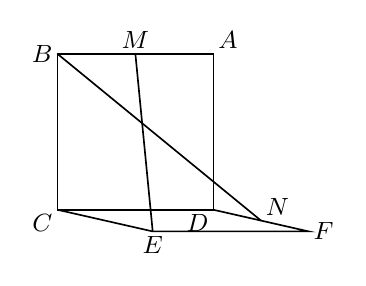
\begin{tikzpicture}[scale=1.1, semithick, every node/.style={inner sep=1.5pt, font=\small}]
  \coordinate (D) at (0,0);
  \coordinate (C) at (-1.8,0);
  \coordinate (B) at (-1.8,1.8);
  \coordinate (A) at (0,1.8);
  \coordinate (E) at (-0.7,-0.25);
  \coordinate (F) at (1.1,-0.25);
  \coordinate (M) at (-0.9,1.8);
  \coordinate (N) at (0.55,-0.125);
  % 竖直正方形 ABCD
  \draw (A) -- (B) -- (C) -- (D) -- cycle;
  % 水平正方形 DCEF
  \draw (C) -- (E) -- (F) -- (D);
  % 图中线段 ME、BN
  \draw (M) -- (E);
  \draw (B) -- (N);
  % 顶点标注
  \node[above right] at (A) {$A$};
  \node[left] at (B) {$B$};
  \node[above] at (M) {$M$};
  \node[below left] at (C) {$C$};
  \node[below left] at (D) {$D$};
  \node[below] at (E) {$E$};
  \node[right] at (F) {$F$};
  \node[above right] at (N) {$N$};
\end{tikzpicture}
\end{center}
\nopagebreak[4]
\Needspace{4\baselineskip}
\textbf{解析}

\Needspace{5\baselineskip}
设正方形边长为 $a$。以 $D$ 为原点，$DC$ 所在直线为 $x$ 轴，平面 $DCEF$ 为 $xOy$ 平面建立空间直角坐标系。因平面 $ABCD\perp$ 平面 $DCEF$，且 $ABCD$ 是以 $CD$ 为一边的正方形，故 $A,B$ 在 $z$ 轴方向高出平面 $DCEF$ 的距离为 $a$：

\nopagebreak[4]
\[D(0,0,0),\quad C(a,0,0),\quad E(a,a,0),\quad F(0,a,0),\]
\nopagebreak[4]
\[A(0,0,a),\quad B(a,0,a).\]

\Needspace{5\baselineskip}
$M$ 为 $AB$ 中点，$N$ 为 $DF$ 中点，故

\nopagebreak[4]
\[M\left(\frac a2,0,a\right),\qquad N\left(0,\frac a2,0\right).\]

\Needspace{5\baselineskip}
（1）直线 $MN$ 的方向向量

\nopagebreak[4]
\[\overrightarrow{NM}=\left(\frac a2,-\frac a2,a\right),\]

\Needspace{5\baselineskip}
其模为

\nopagebreak[4]
\[|\overrightarrow{NM}|
=\sqrt{\frac{a^2}{4}+\frac{a^2}{4}+a^2}
=\sqrt{\frac32}\,a
=\frac{\sqrt6}{2}a .\]

\Needspace{5\baselineskip}
平面 $DCEF$ 就是 $xOy$ 平面，法向量可取 $\boldsymbol n=(0,0,1)$。设 $MN$ 与平面所成角为 $\theta$，则

\nopagebreak[4]
\[\sin\theta
=\frac{|\overrightarrow{NM}\cdot\boldsymbol n|}{|\overrightarrow{NM}||\boldsymbol n|}
=\frac{a}{\frac{\sqrt6}{2}a}
=\frac{2}{\sqrt6}
=\frac{\sqrt6}{3}.\]

（2）用反证法。假设直线 $ME$ 与 $BN$ 共面，则该平面同时含 $M,E,B,N$ 四点。于是从 $M$ 出发的三个向量 $\overrightarrow{MB}$、$\overrightarrow{ME}$、$\overrightarrow{MN}$ 都在同一平面内，其混合积应为零。

\Needspace{5\baselineskip}
由坐标

\nopagebreak[4]
\[\overrightarrow{MB}=\left(\frac a2,0,0\right),\quad
\overrightarrow{ME}=\left(\frac a2,a,-a\right),\quad
\overrightarrow{MN}=\left(-\frac a2,\frac a2,-a\right).\]

\Needspace{5\baselineskip}
计算混合积：

\nopagebreak[4]
\[\det
\begin{pmatrix}
\frac a2&0&0\\
\frac a2&a&-a\\
-\frac a2&\frac a2&-a
\end{pmatrix}
=\frac a2\left(a\cdot(-a)-(-a)\cdot\frac a2\right)
=\frac a2\left(-a^2+\frac{a^2}{2}\right)
=-\frac{a^3}{4}\neq0 .\]

这与“三向量共面”矛盾，故假设不成立，即 $ME$ 与 $BN$ 不共面。两条不共面的直线是异面直线，所证成立。

\gkanswer{答案：（1）$\frac{\sqrt6}{3}$；（2）证明见解析。}

\end{answer}
\begin{answer}
\gksolhead{19}{}

\textbf{题目}：

某人向一目射击 $4$ 次，每次击中目标的概率为 $\frac13$．该目标分为 $3$ 个不同的部分，第一、二、三部分面积之比为 $1:3:6$．击中目标时，击中任何一部分的概率与其面积成正比．

（1）设 $X$ 表示目标被击中的次数，求 $X$ 的分布列；

（2）若目标被击中 $2$ 次，$A$ 表示事件“第一部分至少被击中 $1$ 次或第二部分被击中 $2$ 次”，求 $P(A)$．

\Needspace{4\baselineskip}
\textbf{解析}

每次射击击中目标的概率为 $p=\frac13$，各次射击相互独立。

\Needspace{5\baselineskip}
（1）$X$ 表示 $4$ 次射击中击中目标的次数，故 $X\sim B\left(4,\frac13\right)$，分布列为

\nopagebreak[4]
\[P(X=k)=\mathrm C_4^k\left(\frac13\right)^k\left(\frac23\right)^{4-k},
\qquad k=0,1,2,3,4 .\]

\Needspace{5\baselineskip}
逐项计算：

\nopagebreak[4]
\[P(X=0)=\left(\frac23\right)^4=\frac{16}{81},\]
\nopagebreak[4]
\[P(X=1)=4\cdot\frac13\cdot\left(\frac23\right)^3=\frac{32}{81},\]
\nopagebreak[4]
\[P(X=2)=6\cdot\left(\frac13\right)^2\left(\frac23\right)^2=\frac{24}{81},\]
\nopagebreak[4]
\[P(X=3)=4\cdot\left(\frac13\right)^3\cdot\frac23=\frac{8}{81},\]
\nopagebreak[4]
\[P(X=4)=\left(\frac13\right)^4=\frac{1}{81}.\]

检验：$\frac{16+32+24+8+1}{81}=\frac{81}{81}=1$。

\Needspace{5\baselineskip}
（2）三部分面积比为 $1:3:6$，击中任一部分的概率与面积成正比，故在“击中目标”的条件下，每次击中第一、二、三部分的概率分别为

\nopagebreak[4]
\[p_1=\frac1{10},\qquad p_2=\frac3{10},\qquad p_3=\frac6{10}.\]

\Needspace{5\baselineskip}
已知目标被击中 $2$ 次，这两次落点相互独立。记 $N_i$ 为这两次中击中第 $i$ 部分的次数，则

\nopagebreak[4]
\[P(N_1\geqslant1)=1-P(N_1=0)
=1-\left(\frac9{10}\right)^2
=\frac{19}{100},\]

\nopagebreak[4]
\[P(N_2=2)=\left(\frac3{10}\right)^2=\frac9{100}.\]

\Needspace{5\baselineskip}
在总共只有 $2$ 次击中的条件下，事件“$N_1\geqslant1$”与“$N_2=2$”不能同时发生（前者至少占用一次击中，后者占用全部两次且都落在第二部分），故

\nopagebreak[4]
\[P(A)=P(N_1\geqslant1)+P(N_2=2)
=\frac{19}{100}+\frac9{100}
=\frac{28}{100}
=\frac7{25}.\]

\gkanswer{答案：（1）$P(X=k)=\mathrm C_4^k\left(\frac13\right)^k\left(\frac23\right)^{4-k}$（$k=0,1,2,3,4$）；（2）$\frac7{25}$。}

\end{answer}
\begin{answer}
\gksolhead{20}{}

\textbf{题目}：

已知椭圆 $C$ 过点 $A\left(1,\frac32\right)$，两个焦点为 $(-1,0)$，$(1,0)$．

（1）求椭圆 $C$ 的方程；

（2）$E,F$ 是椭圆 $C$ 上的两个动点，如果直线 $AE$ 的斜率与 $AF$ 的斜率互为相反数，证明直线 $EF$ 的斜率为定值，并求出这个定值．

\Needspace{4\baselineskip}
\textbf{解析}

\Needspace{5\baselineskip}
（1）设椭圆方程为 $\frac{x^2}{a^2}+\frac{y^2}{b^2}=1$（$a>b>0$）。两焦点为 $(-1,0)$、$(1,0)$，故半焦距 $c=1$，且

\nopagebreak[4]
\[a^2=b^2+c^2=b^2+1 .\]

\Needspace{5\baselineskip}
代入点 $A\left(1,\frac32\right)$：

\nopagebreak[4]
\[\frac{1}{b^2+1}+\frac{9}{4b^2}=1 .\]

\Needspace{5\baselineskip}
两边乘 $4b^2(b^2+1)$：

\nopagebreak[4]
\[4b^2+9(b^2+1)=4b^2(b^2+1),\]

\Needspace{5\baselineskip}
即

\nopagebreak[4]
\[4b^4+4b^2-4b^2-9b^2-9=0
\ \Longrightarrow\ 4b^4-9b^2-9=0 .\]

\Needspace{5\baselineskip}
令 $t=b^2>0$，解 $4t^2-9t-9=0$：

\nopagebreak[4]
\[t=\frac{9\pm\sqrt{81+144}}{8}
=\frac{9\pm15}{8},\]

\Needspace{5\baselineskip}
正根 $t=3$，故 $b^2=3$、$a^2=4$，椭圆为

\nopagebreak[4]
\[C:\ \frac{x^2}{4}+\frac{y^2}{3}=1 .\]

\Needspace{5\baselineskip}
（2）设直线 $AE$ 的斜率为 $k$，则 $AF$ 的斜率为 $-k$。过 $A\left(1,\frac32\right)$ 的直线 $AE$ 为

\nopagebreak[4]
\[y=k(x-1)+\frac32=kx+\left(\frac32-k\right).\]

\Needspace{5\baselineskip}
代入椭圆方程 $3x^2+4y^2=12$，得关于 $x$ 的二次方程。记 $m=\frac32-k$，则

\nopagebreak[4]
\[3x^2+4(kx+m)^2=12,\]

\Needspace{5\baselineskip}
即

\nopagebreak[4]
\[(3+4k^2)x^2+8km\,x+4m^2-12=0 .\]

\Needspace{5\baselineskip}
因为 $A$ 在椭圆上，$x=1$ 是该方程的一个根；由韦达定理，两根之积为 $\frac{4m^2-12}{3+4k^2}$，故另一根

\nopagebreak[4]
\[x_E=\frac{4m^2-12}{3+4k^2}\cdot\frac1{1}
=\frac{4\left(\frac32-k\right)^2-12}{3+4k^2}
=\frac{4k^2-12k-3}{3+4k^2}.\]

\Needspace{5\baselineskip}
把 $k$ 换成 $-k$，得 $F$ 的横坐标

\nopagebreak[4]
\[x_F=\frac{4k^2+12k-3}{3+4k^2}.\]

\Needspace{5\baselineskip}
于是

\nopagebreak[4]
\[x_E-x_F=\frac{-24k}{3+4k^2}.\]

\Needspace{5\baselineskip}
又 $E,F$ 都在相应直线上，

\nopagebreak[4]
\[y_E=kx_E+\frac32-k,\qquad
y_F=-kx_F+\frac32+k,\]

\Needspace{5\baselineskip}
相减得

\nopagebreak[4]
\[y_E-y_F
=k(x_E+x_F)-2k .\]

\Needspace{5\baselineskip}
而

\nopagebreak[4]
\[x_E+x_F
=\frac{8k^2-6}{3+4k^2}
=\frac{2(4k^2-3)}{3+4k^2},\]

\Needspace{5\baselineskip}
故

\nopagebreak[4]
\[y_E-y_F
=k\cdot\frac{2(4k^2-3)}{3+4k^2}-2k
=\frac{2k(4k^2-3)-2k(3+4k^2)}{3+4k^2}
=\frac{-12k}{3+4k^2}.\]

\Needspace{5\baselineskip}
因此

\nopagebreak[4]
\[k_{EF}
=\frac{y_E-y_F}{x_E-x_F}
=\frac{-12k}{-24k}
=\frac12,\]

即直线 $EF$ 的斜率为定值 $\frac12$（$k\neq0$；若 $k=0$ 则 $E,F$ 重合，不合题意）。

\gkanswer{答案：（1）$\frac{x^2}{4}+\frac{y^2}{3}=1$；（2）定值为 $\frac12$。}

\end{answer}
\begin{answer}
\gksolhead{21}{}

\textbf{题目}：

已知函数 $f(x)=\frac12x^2-ax+(a-1)\ln x$，$a>1$．

（1）讨论函数 $f(x)$ 的单调性；

\Needspace{5\baselineskip}
（2）证明：若 $a<5$，则对于任意 $x_1,x_2\in(0,+\infty)$，$x_1\neq x_2$，有

\nopagebreak[4]
\[\frac{f(x_1)-f(x_2)}{x_1-x_2}>-1 .\]

\Needspace{4\baselineskip}
\textbf{解析}

\Needspace{5\baselineskip}
（1）函数的定义域为 $(0,+\infty)$。求导：

\nopagebreak[4]
\[f'(x)=x-a+\frac{a-1}{x}
=\frac{x^2-ax+a-1}{x}
=\frac{(x-1)(x-a+1)}{x}.\]

因 $a>1$，故 $a-1>0$，分母 $x>0$，$f'(x)$ 的符号由分子 $(x-1)(x-(a-1))$ 决定。按 $a-1$ 与 $1$ 的大小分三种情形。

当 $1<a<2$ 时，$0<a-1<1$。在 $(0,a-1)$ 上两根式均为负、乘积为正；在 $(a-1,1)$ 上乘积为负；在 $(1,+\infty)$ 上乘积为正。故 $f(x)$ 在 $(0,a-1)$ 与 $(1,+\infty)$ 上单调递增，在 $(a-1,1)$ 上单调递减。

\Needspace{5\baselineskip}
当 $a=2$ 时，$a-1=1$，

\nopagebreak[4]
\[f'(x)=\frac{(x-1)^2}{x}\geqslant0,\]

故 $f(x)$ 在 $(0,+\infty)$ 上单调递增。

当 $a>2$ 时，$a-1>1$。同理，$f(x)$ 在 $(0,1)$ 与 $(a-1,+\infty)$ 上单调递增，在 $(1,a-1)$ 上单调递减。

\Needspace{5\baselineskip}
（2）要证对任意 $x_1\neq x_2$ 有 $\frac{f(x_1)-f(x_2)}{x_1-x_2}>-1$，等价于证明函数

\nopagebreak[4]
\[g(x)=f(x)+x\]

\Needspace{5\baselineskip}
在 $(0,+\infty)$ 上严格递增，因为

\nopagebreak[4]
\[\frac{g(x_1)-g(x_2)}{x_1-x_2}
=\frac{f(x_1)-f(x_2)}{x_1-x_2}+1 .\]

\Needspace{5\baselineskip}
求导：

\nopagebreak[4]
\[g'(x)=f'(x)+1
=x-a+\frac{a-1}{x}+1
=\frac{x^2+(1-a)x+(a-1)}{x}.\]

\Needspace{5\baselineskip}
分子的判别式为

\nopagebreak[4]
\[\Delta=(1-a)^2-4(a-1)
=(a-1)^2-4(a-1)
=(a-1)(a-5).\]

\Needspace{5\baselineskip}
当 $1<a<5$ 时，$a-1>0$、$a-5<0$，故 $\Delta<0$；又分子是开口向上的二次式，所以对一切实数 $x$ 都有

\nopagebreak[4]
\[x^2+(1-a)x+(a-1)>0 .\]

\Needspace{5\baselineskip}
结合 $x>0$，得 $g'(x)>0$，故 $g$ 在 $(0,+\infty)$ 上严格递增。于是对 $x_1\neq x_2$，

\nopagebreak[4]
\[\frac{g(x_1)-g(x_2)}{x_1-x_2}>0
\ \Longrightarrow\ \frac{f(x_1)-f(x_2)}{x_1-x_2}>-1 .\]

\gkanswer{答案：（1）按 $1<a<2$、$a=2$、$a>2$ 分列单调区间；（2）证明见解析。}

\end{answer}
\begin{answer}
\gksolhead{22}{}

\textbf{题目}：

三选一．

\textbf{【A】} 已知 $\triangle ABC$ 中，$AB=AC$，$D$ 是 $\triangle ABC$ 外接圆劣弧 $\overset{\frown}{AC}$ 上的点（不与点 $A,C$ 重合），延长 $BD$ 至 $E$．

（1）求证：$AD$ 的延长线平分 $\angle CDE$；

（2）若 $\angle BAC=30^\circ$，$\triangle ABC$ 中 $BC$ 边上的高为 $2+\sqrt3$，求 $\triangle ABC$ 外接圆的面积．

\textbf{【B】} 在直角坐标系 $xOy$ 中，以 $O$ 为极点，$x$ 正半轴为极轴建立极坐标系，曲线 $C$ 的极坐标方程为 $\rho\cos\left(\theta-\frac{\pi}{3}\right)=1$，$M,N$ 分别为 $C$ 与 $x$ 轴、$y$ 轴的交点．

（1）写出 $C$ 的直角坐标方程，并求 $M,N$ 的极坐标；

（2）设 $MN$ 的中点为 $P$，求直线 $OP$ 的极坐标方程．

\textbf{【C】} 设函数 $f(x)=|x-1|+|x-a|$．

（1）若 $a=-1$，解不等式 $f(x)\geqslant3$；

（2）如果 $\forall x\in\mathbf R$，$f(x)\geqslant2$，求 $a$ 的取值范围．
\nopagebreak[4]
\begin{center}% 2009 年辽宁卷理科第 22 题【A】：△ABC 的外接圆，D 是劣弧 AC 上的点，延长 BD 至 E。
% 来源 PDF：普通高考/2009/2009辽宁理.pdf，SHA256 5ae9708acfe7def5bddd60a34d1474cfa2e2c20a39d130255e0e4393093accad
% 原页：第 2 页（A3 三栏）第 3 栏上部，印刷页 538。
% 重绘依据：A 在圆上最高处，B、C 在下方左右对称（AB=AC），D 在 A 与 C 之间的劣弧上，
%   B、D、E 共线且 E 在 D 的延长线上；连 AB、AC、AD、BC、CD，并延长 BD 至 E。
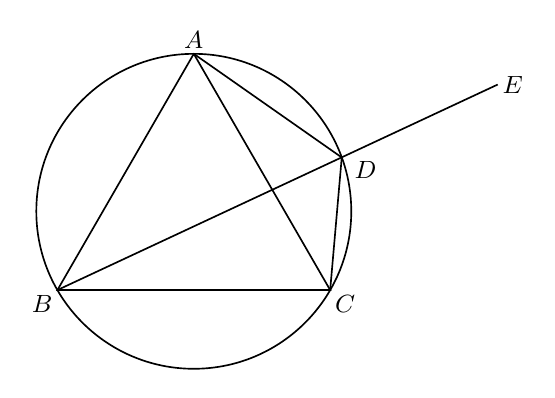
\begin{tikzpicture}[scale=1.0, semithick, every node/.style={inner sep=1.5pt, font=\small}]
  \coordinate (O) at (0,0);
  \coordinate (A) at (0,2);
  \coordinate (B) at (-1.732,-1);
  \coordinate (C) at (1.732,-1);
  \coordinate (D) at (1.879,0.684);
  \coordinate (E) at (3.86,1.61);
  % 外接圆
  \draw (O) circle (2);
  % 三角形与相关线段
  \draw (A) -- (B) -- (C) -- (A);
  \draw (A) -- (D);
  \draw (C) -- (D);
  \draw (B) -- (E);
  % 顶点标注
  \node[above] at (A) {$A$};
  \node[below left] at (B) {$B$};
  \node[below right] at (C) {$C$};
  \node[right] at (1.98,0.52) {$D$};
  \node[right] at (E) {$E$};
\end{tikzpicture}
\end{center}
\nopagebreak[4]
\Needspace{4\baselineskip}
\textbf{解析}

本题为三选一，下面分别给出【A】【B】【C】的解答。

\Needspace{5\baselineskip}
\textbf{【A】}（1）设 $F$ 为 $AD$ 的延长线上、$D$ 之外的一点。因为 $A,B,C,D$ 四点共圆，圆内接四边形对角互补：

\nopagebreak[4]
\[\angle CDA+\angle CBA=180^\circ .\]

\Needspace{5\baselineskip}
而 $F,D,A$ 共线，$\angle CDF$ 与 $\angle CDA$ 互补，故

\nopagebreak[4]
\[\angle CDF=180^\circ-\angle CDA=\angle CBA .\]

\Needspace{5\baselineskip}
又 $E,D,B$ 共线且 $E$ 在 $BD$ 的延长线上，$F,D,A$ 共线，故 $\angle FDE$ 与 $\angle ADB$ 是对顶角：

\nopagebreak[4]
\[\angle FDE=\angle ADB .\]

\Needspace{5\baselineskip}
同弧 $AB$ 所对的圆周角相等，$\angle ADB=\angle ACB$。由 $AB=AC$ 得 $\angle ABC=\angle ACB$，从而

\nopagebreak[4]
\[\angle CDF=\angle CBA=\angle ACB=\angle ADB=\angle FDE .\]

即 $AD$ 的延长线 $DF$ 平分 $\angle CDE$。

\Needspace{5\baselineskip}
（2）设 $BC$ 的中点为 $H$，$BC$ 边上的高 $AH=h=2+\sqrt3$。由 $AB=AC$，$AH$ 垂直平分 $BC$，且 $\angle BAH=\frac12\angle BAC=15^\circ$。于是

\nopagebreak[4]
\[\frac{BC}{2}=BH=AH\tan15^\circ
=(2+\sqrt3)(2-\sqrt3)=1,\]

故 $BC=2$。

\Needspace{5\baselineskip}
由正弦定理，$\triangle ABC$ 外接圆半径 $R$ 满足

\nopagebreak[4]
\[2R=\frac{BC}{\sin\angle BAC}
=\frac{2}{\sin30^\circ}=4,\]

\Needspace{5\baselineskip}
故 $R=2$，外接圆面积为

\nopagebreak[4]
\[S=\pi R^2=4\pi .\]

\Needspace{5\baselineskip}
\textbf{【B】}（1）极坐标与直角坐标的关系为 $x=\rho\cos\theta$、$y=\rho\sin\theta$。展开

\nopagebreak[4]
\[\rho\cos\left(\theta-\frac\pi3\right)
=\rho\left(\cos\theta\cos\frac\pi3+\sin\theta\sin\frac\pi3\right)
=\frac12x+\frac{\sqrt3}{2}y,\]

\Needspace{5\baselineskip}
故曲线 $C$ 的直角坐标方程为

\nopagebreak[4]
\[\frac12x+\frac{\sqrt3}{2}y=1,
\quad\text{\text{即}}\quad x+\sqrt3y=2 .\]

与 $x$ 轴的交点：令 $y=0$，得 $x=2$，故 $M(2,0)$，其极坐标为 $\rho=2$、$\theta=0$，即 $(2,0)$。

与 $y$ 轴的交点：令 $x=0$，得 $y=\frac{2}{\sqrt3}=\frac{2\sqrt3}{3}$，故 $N\left(0,\frac{2\sqrt3}{3}\right)$，其极坐标为 $\rho=\frac{2\sqrt3}{3}$、$\theta=\frac\pi2$，即 $\left(\frac{2\sqrt3}{3},\frac\pi2\right)$。

\Needspace{5\baselineskip}
（2）$MN$ 的中点

\nopagebreak[4]
\[P\left(\frac{2+0}{2},\frac{0+\frac{2\sqrt3}{3}}{2}\right)
=\left(1,\frac{\sqrt3}{3}\right).\]

\Needspace{5\baselineskip}
直线 $OP$ 过原点与 $P$，斜率为

\nopagebreak[4]
\[\frac{\frac{\sqrt3}{3}}{1}=\frac{\sqrt3}{3}=\tan\frac\pi6 .\]

\Needspace{5\baselineskip}
故直线 $OP$ 的极坐标方程为

\nopagebreak[4]
\[\theta=\frac\pi6\quad(\rho\in\mathbf R).\]

\Needspace{5\baselineskip}
\textbf{【C】}（1）当 $a=-1$ 时，

\nopagebreak[4]
\[f(x)=|x-1|+|x+1| .\]

按零点 $-1,1$ 分段：

\begin{itemize}
\item 当 $x\leqslant-1$ 时，$f(x)=-(x-1)-(x+1)=-2x$，由 $-2x\geqslant3$ 得 $x\leqslant-\frac32$；
\item 当 $-1<x<1$ 时，$f(x)=-(x-1)+(x+1)=2$，不满足 $2\geqslant3$；
\item 当 $x\geqslant1$ 时，$f(x)=(x-1)+(x+1)=2x$，由 $2x\geqslant3$ 得 $x\geqslant\frac32$。
\end{itemize}

\Needspace{5\baselineskip}
故解集为

\nopagebreak[4]
\[\left(-\infty,-\frac32\right]\cup\left[\frac32,+\infty\right).\]

\Needspace{5\baselineskip}
（2）由绝对值不等式，

\nopagebreak[4]
\[f(x)=|x-1|+|x-a|\geqslant|(x-1)-(x-a)|=|a-1| .\]

\Needspace{5\baselineskip}
当 $x$ 介于 $1$ 与 $a$ 之间时取等号，故 $f$ 的最小值为 $|a-1|$。题设要求对任意 $x\in\mathbf R$ 都有 $f(x)\geqslant2$，等价于

\nopagebreak[4]
\[|a-1|\geqslant2 .\]

\Needspace{5\baselineskip}
解得 $a-1\geqslant2$ 或 $a-1\leqslant-2$，即

\nopagebreak[4]
\[a\geqslant3\quad\text{\text{或}}\quad a\leqslant-1 .\]

\gkanswer{答案：【A】（1）证明见解析；（2）$4\pi$；【B】（1）$x+\sqrt3y=2$，$M(2,0)$，$N\left(\frac{2\sqrt3}{3},\frac\pi2\right)$；（2）$\theta=\frac\pi6$；【C】（1）$\left(-\infty,-\frac32\right]\cup\left[\frac32,+\infty\right)$；（2）$a\leqslant-1$ 或 $a\geqslant3$。}

\end{answer}